\let\negmedspace\undefined
\let\negthickspace\undefined
\documentclass[journal,12pt,onecolumn]{IEEEtran}
\usepackage{pgfplots}
\pgfplotsset{compat=1.17}
\usepackage{cite}
\usepackage{amsmath,amssymb,amsfonts,amsthm}
\usepackage{algorithmic}
\usepackage{graphicx}
\usepackage{textcomp}
\usepackage{xcolor}
\usepackage{txfonts}
\usepackage{listings}
\usepackage{enumitem}
\usepackage{mathtools}
\usepackage{gensymb}
\usepackage{comment}
\usepackage[breaklinks=true]{hyperref}
\usepackage{tkz-euclide} 
\usepackage{listings}
\usepackage{gvv}                                        
\def\inputGnumericTable{}                                 
\usepackage[latin1]{inputenc}                                
\usepackage{color}                                            
\usepackage{array}                                            
\usepackage{longtable}                                       
\usepackage{calc}                                             
\usepackage{multirow}                                         
\usepackage{hhline}                                           
\usepackage{ifthen}                                           
\usepackage{lscape}
\newtheorem{theorem}{Theorem}[section]
\newtheorem{problem}{Problem}
\newtheorem{proposition}{Proposition}[section]
\newtheorem{lemma}{Lemma}[section]
\newtheorem{corollary}[theorem]{Corollary}
\newtheorem{example}{Example}[section]
\newtheorem{definition}[problem]{Definition}
\newcommand{\BEQA}{\begin{eqnarray}}
\newcommand{\EEQA}{\end{eqnarray}}
\newcommand{\define}{\stackrel{\triangle}{=}}
\theoremstyle{remark}
\newtheorem{rem}{Remark}
\begin{document}
\bibliographystyle{IEEEtran}
\vspace{3cm}
\title{GATE GE 81Q}
\author{EE23BTECH11021 - GANNE GOPI CHANDU$^{*}$% <-this % stops a space
}
\maketitle
\bigskip
\renewcommand{\thefigure}{\theenumi}
\renewcommand{\thetable}{\theenumi}
\bibliographystyle{IEEEtran}
\textbf{Question}\\
The value of the convolution of $f(x) = 3\cos(2x)$ and $g(x) = \frac{1}{3}\sin(2x)$ where $x \in [0, 2\pi)$, at $x = \frac{\pi}{3}$, is (Rounded off to 2 decimal places)\\
\textbf{Solution}\\

The f(x) = $3\cos(2x)$ the  Fourier series is
\begin{align}
    c\brak{n1}&=\frac{1}{p}\int_{0}^{2\pi}f\brak{x}e^{-j\frac{2\pi n x}{p}}\;dx \\
    &=\frac{3}{2\pi}\int_{0}^{2\pi}\cos\brak{2x}e^{-j\frac{\pi n x}{\pi}}\;dx \\
    &=\frac{3}{2\pi}\int_{0}^{2\pi}\cos\brak{2x}\brak{\cos\brak{nx}-j\sin\brak{nx}}\;dx \\
    &=\frac{3}{2\pi}\int_{0}^{2\pi}\cos\brak{2x}\cos\brak{nx}-j\cos\brak{2x}\sin\brak{nx}\;dx \\
    &=\frac{3}{2\pi}\int_{0}^{2\pi}\frac{1}{2}\brak{\cos\brak{\brak{2+n}x}+\brak{\cos\brak{\brak{2-n}x}}}-j\brak{\sin\brak{\brak{2+n}x}-\sin\brak{2-n}x}\;dx \\
    &=0 \quad{n1\neq-2,2}
\end{align}
Except c1\brak{-2},c1\brak{2} remaining all values are 0
\begin{align}
    c1\brak{2}&=\frac{3}{2\pi}\int_{0}^{2\pi}\cos\brak{2x}e^{-j\brak{\pi 2 x}}\;dx \\
    &=\frac{3}{2\pi}\int_{0}^{2\pi}\cos\brak{2x}\brak{\cos\brak{2x}-j\sin\brak{2x}}\;dx \\
    &=\frac{3}{2\pi}\int_{0}^{2\pi}\cos^2\brak{2x}-j\sin\brak{2x}\cos\brak{2x}\;dx \\
    &=\frac{3}{2\pi}\brak{\frac{2\pi}{2}}\\
    c1\brak{2}&=\frac{3}{2}
\end{align}
and
\begin{align}
    c1\brak{-2}&=\frac{3}{2\pi}\int_{0}^{2\pi}\cos\brak{2x}e^{j\brak{\pi 2 x}}\;dx \\
    &=\frac{3}{2\pi}\int_{0}^{2\pi}\cos\brak{2x}\brak{\cos\brak{2x}+j\sin\brak{2x}}\;dx \\
    &=\frac{3}{2\pi}\int_{0}^{2\pi}\cos^2\brak{2x}+j\sin\brak{2x}\cos\brak{2x}\;dx \\
    &=\frac{3}{2\pi}\brak{\frac{2\pi-0}{2}}\\
    c1\brak{-2}&=\frac{3}{2}
\end{align}
 For $ g(x) = \frac{1}{3}\sin(2x) $ the Fourier series is:
 \begin{align}
    c2\brak{n2}&=\frac{1}{p}\int_{0}^{2\pi}g\brak{x}e^{-j\frac{2\pi n x}{p}}\;dx \\
    &=\frac{1}{6\pi}\int_{0}^{2\pi}\sin\brak{2x}e^{-j\frac{\pi n x}{\pi}}\;dx \\
    &=\frac{1}{6\pi}\int_{0}^{2\pi}\sin\brak{2x}\brak{\cos\brak{nx}-j\sin\brak{nx}}\;dx \\
    &=\frac{1}{6\pi}\int_{0}^{2\pi}\sin\brak{2x}\cos\brak{nx}-j\sin\brak{2x}\sin\brak{nx}\;dx \\
    &=\frac{1}{6\pi}\int_{0}^{2\pi}\frac{1}{2}\brak{\sin\brak{\brak{2+n}x}+\brak{\sin\brak{\brak{2-n}x}}}-j\brak{\cos\brak{\brak{2-n}x}-\cos\brak{2+n}x}\;dx \\
    &=0 \quad{n2\neq-2,2}
\end{align}
Except c2\brak{-2},c2\brak{2} remaining all values are 0
\begin{align}
    c2\brak{2}&=\frac{1}{6\pi}\int_{0}^{2\pi}\sin\brak{2x}e^{-j\brak{\pi 2 x}}\;dx \\
    &=\frac{1}{6\pi}\int_{0}^{2\pi}\sin\brak{2x}\brak{\cos\brak{2x}-j\sin\brak{2x}}\;dx \\
    &=\frac{1}{6\pi}\int_{0}^{2\pi}\sin\brak{2x}\cos\brak{2x}-j\sin^2\brak{2x}\;dx \\
    &=\frac{1}{6\pi}\brak{\frac{2\pi-0}{2}}\brak{-j}\\
    &=\frac{-j}{6}\\
\end{align}
and
\begin{align}
    c2\brak{-2}&=\frac{1}{6\pi}\int_{0}^{2\pi}\sin\brak{2x}e^{j\brak{\pi 2 x}}\;dx \\
    &=\frac{1}{6\pi}\int_{0}^{2\pi}\sin\brak{2x}\brak{\cos\brak{2x}+j\sin\brak{2x}}\;dx \\
    &=\frac{1}{6\pi}\int_{0}^{2\pi}\sin\brak{2x}\cos\brak{2x}+j\sin^2\brak{2x}\;dx \\
    &=\frac{1}{6\pi}\brak{\frac{2\pi}{2}}\brak{j}\\
    &=\frac{j}{6}
\end{align}
By periodic convolution with Fourier series coefficients is
\brak{n}=c\brak{n1}*c\brak{n2}*p\\
\begin{align}
    c\brak{2}&=c1\brak{2}*c2\brak{2}*p\\
    &=\brak{\frac{3}{2}}\brak{\frac{-j}{6}}\brak{2\pi}\\
    &=\frac{-j\pi}{2}
\end{align}
and
\begin{align}
    c\brak{-2}&=c1\brak{-2}*c2\brak{-2}*p\\
    &=\brak{\frac{3}{2}}\brak{\frac{j}{6}}\brak{2\pi}\\
    &=\frac{j\pi}{2}
\end{align}
\begin{align}
   {f*g}\brak{x}&=\sum_{n=-N}^{N}c\brak{n} e^{j\frac{\pi nx}{L}}\\
    &=c\brak{-2}e^{-j2x} + c\brak{2}e^{j2x}\\
    &=\frac{j\pi}{2}e^{-j2x}-\frac{j\pi}{2}e^{j2x}\\
    &=\frac{-j\pi}{2}\brak{e^{j2x}-e^{-j2x}}\\
    &=\frac{-j\pi}{2}\brak{sin\brak{2x}2j}\\
    &=\pi \sin\brak{2x}\\
\end{align}
at $x=\frac{\pi}{3}$
\begin{align}
    &=\frac{\sqrt{3}\pi}{2}\\
    &=2.72
\end{align}
Therefore the convolution of f(x) and g(x) is 2.72
\begin{figure}[!h]
    \centering
    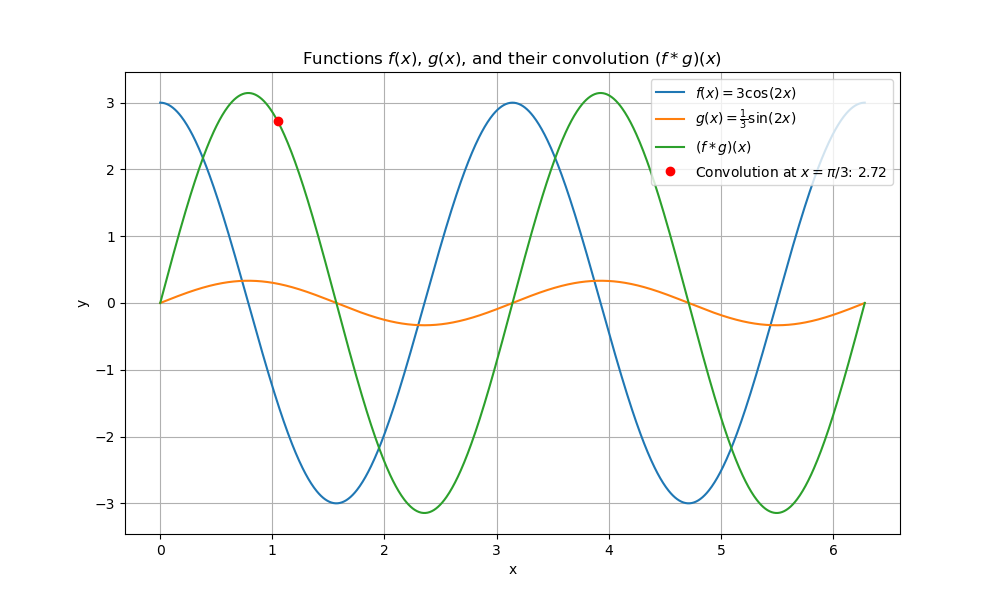
\includegraphics[width=1.0\linewidth]{ga.81.png}
    \caption{Plot of y vs x}
    \label{fig:1}
\end{figure}
For $n\neq0$,
\end{document}
